\section{Methods}

%\subsection{Existing methods}
%We found no existing methods for authentication via. Bluetooth RSSI values.

\subsection{Proposed method}

The proposed method overview is presented on \cref{fig_solution_overview}. A "Base station" is a stationary device, which authenticates the user.

The base station reads the RSSI value from the Phone's BLE signal and uses a median filter to filter the values. A hysteresis threshold is added in order to determine if the user should change state to logged out, logged in or no change.

The following explains the components in detail.

\subsubsection{RSSI for proximity detection}

RSSI measures the signal quality between 2 transmitters.
The signal quality is dependent on multiple factors among witch are signal reflections form the environment, transmission strength, antenna and finally distance. 
It is hard if not impossible to isolate the change in RSSI caused by a change in distance.
However if exact distance is not necessary and knowledge of environment and devices are available, then devices can be calibrated with thresholds and used for detecting proximity.

% % TODO remove, is replace by the above % %
%It is hard to convert RSSI values into distance because of it's fluctuating nature and the effect of the surrounding environment.
%Thus instead of dealing in distances the way proximity is detected in this system is by a predefined RSSI value threshold.
%By determining this threshold and using filters to remove noise it is possible to use RSSI as a means for proximity detection.

\begin{figure}[!t]
	\centering
	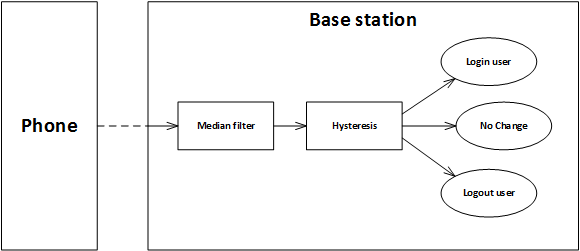
\includegraphics[width=3.5in]{img/SolutionOverview}
	\caption{ Proposed method overview }
	\label{fig_solution_overview}
\end{figure}

%\begin{figure}[!t]
%	\centering
%	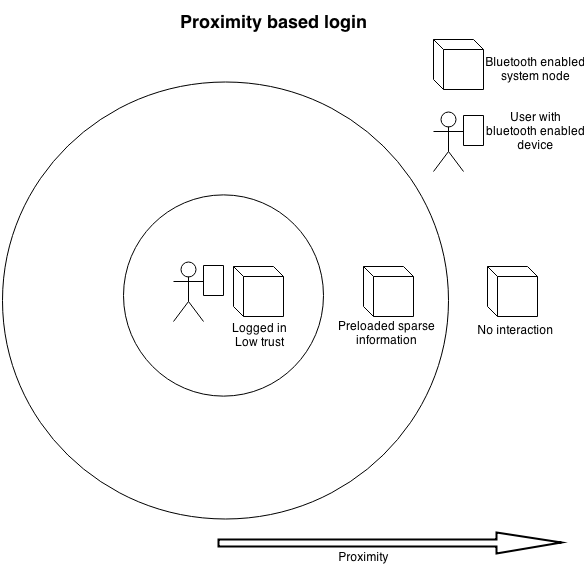
\includegraphics[width=2.5in]{img/proximityBasedLogin}
%	\caption{ Proximity based login }
%	\label{fig_proximity_based_login}
%\end{figure}

% % TODO remove, is not part of our system % %
% Furthermore it is possible to preload information about earlier sessions when a user is moving towards the system.
% When the user is close enough to be partially authenticated the system thus has preloaded information and may be able to present additional relevant data based on the preloaded information from earlier sessions. 
% \cref{fig_proximity_based_login} illustrates the concept of preloading information based on the users proximity to the system.

\subsubsection{Noise reduction filter}
In order to reduce the noise of the RSSI measurements a standard median-filter was added to the system.
When looking at the results plotted in \cref{graf_InsideMesurements} we see some noise with a few extreme values.
The extreme values must be filtered. Both a median and a mean can do this but with a median filter these values can be filtered completely out and does not register in the output. Any small deviations normally handled by a mean filter will be handled by the hysteresis threshold.

\subsubsection{Hysteresis thresholds}
When the strength of the filtered RSSI signal reaches the predefined upper threshold, the user is sufficiently close to interact with the system, and the user will be partially authenticated.
When a user has been authenticated but decides to move away from the system the user will be de-authenticated when the RSSI reaches a predefined lower threshold.
This prevents the user from being constantly logged in and out when the RSSI value is close to a single threshold.

\subsection{Bluetooth Low Energy authentication}
